\documentclass[conference]{IEEEtran}
\IEEEoverridecommandlockouts
% The preceding line is only needed to identify funding in the first footnote. If that is unneeded, please comment it out.
\usepackage{cite}
\usepackage{amsmath,amssymb,amsfonts}
\usepackage{algorithmic}
\usepackage{graphicx}
\usepackage{textcomp}
\usepackage{xcolor}
\usepackage{ctex}
\usepackage{fontspec}

\def\BibTeX{{\rm B\kern-.05em{\sc i\kern-.025em b}\kern-.08em
    T\kern-.1667em\lower.7ex\hbox{E}\kern-.125emX}}
\begin{document}

\title{傅立叶变换光谱测量技术实验报告}

\author{
    \IEEEauthorblockN{
        黄润华}
        \IEEEauthorblockA{
            \textit{Ocean University of China} \\
            \textit{email@noreply.com}
    \and
    \IEEEauthorblockN{
        杨超}
        \IEEEauthorblockA{
            \textit{Ocean University of China} \\
            \textit{email@somewhere.com}
        }
    }
}

\maketitle

\begin{abstract}
    本实验报告为傅立叶变换光谱测量技术第三次实验报告,本报告采用Python仿真对干涉波形补零与加窗环境下的傅里叶变换光谱测量系统的FFT曲线。中心波长选择632.8nm。
\end{abstract}

\begin{IEEEkeywords}
    Optical spectrum, python, fft
\end{IEEEkeywords}

\section{实验目的}
\begin{itemize}
    \item 仿真干涉图补零对光谱曲线的影响
    \item 探索干涉图加不同窗后补零对光谱曲线的影响
\end{itemize}

\section{实验原理}

\subsection{分辨率和分辨能力}

光谱分辨率R由下式定义
\begin{align}
    R = \frac{\sigma_{max}}{\delta \sigma}
\end{align}
其中$\sigma_{max}$是光谱仪设计运行的最大波数。

理论上,单色光的干涉图的表达式如下
\begin{align}
    I(x) = 2cos(2\pi \sigma_0 x)
\end{align}

\subsection{补零与加窗的影响}
对一段曲线补零最直接的影响为提高了该曲线的FFT分辨率,补零操作可以使得FFT之后的曲线变得更加光滑。但由于补零并没有对实际测量的光的长度增加影响,因此补零操作无法改变原始波形分辨率(光谱分辨率),即由于采样长度的不足导致的FFT曲线中两个相邻的峰无法区分开,通过对函数补零操作依旧打不到区分两个相邻峰的目的。补零在时域上相当于对曲线加矩形窗,该矩形窗的FFT变换为$sinc$函数,具备很多个旁瓣,因此补零后的FFT曲线会产生多个旁瓣。

加窗最直接的作用在于消除补零后曲线出现的各种各样的旁瓣。但由于旁瓣被消除,因此旁瓣的能量都集中到主峰上,导致主峰出现FWHM加宽的现象。


\section{实验内容}
\begin{itemize}
    \item[1.] 仿真对于干涉图补零后的傅里叶变换FFT曲线,观察其变化。
    \item[2.] 仿真对于干涉图加窗函数并补零后的傅里叶变换FFT曲线,观察期变化。(以632.8nm的He-Ne激光为例,光程差采样间隔为79.1nm)
\end{itemize}

\begin{figure*}[htbp]
	\centerline{
		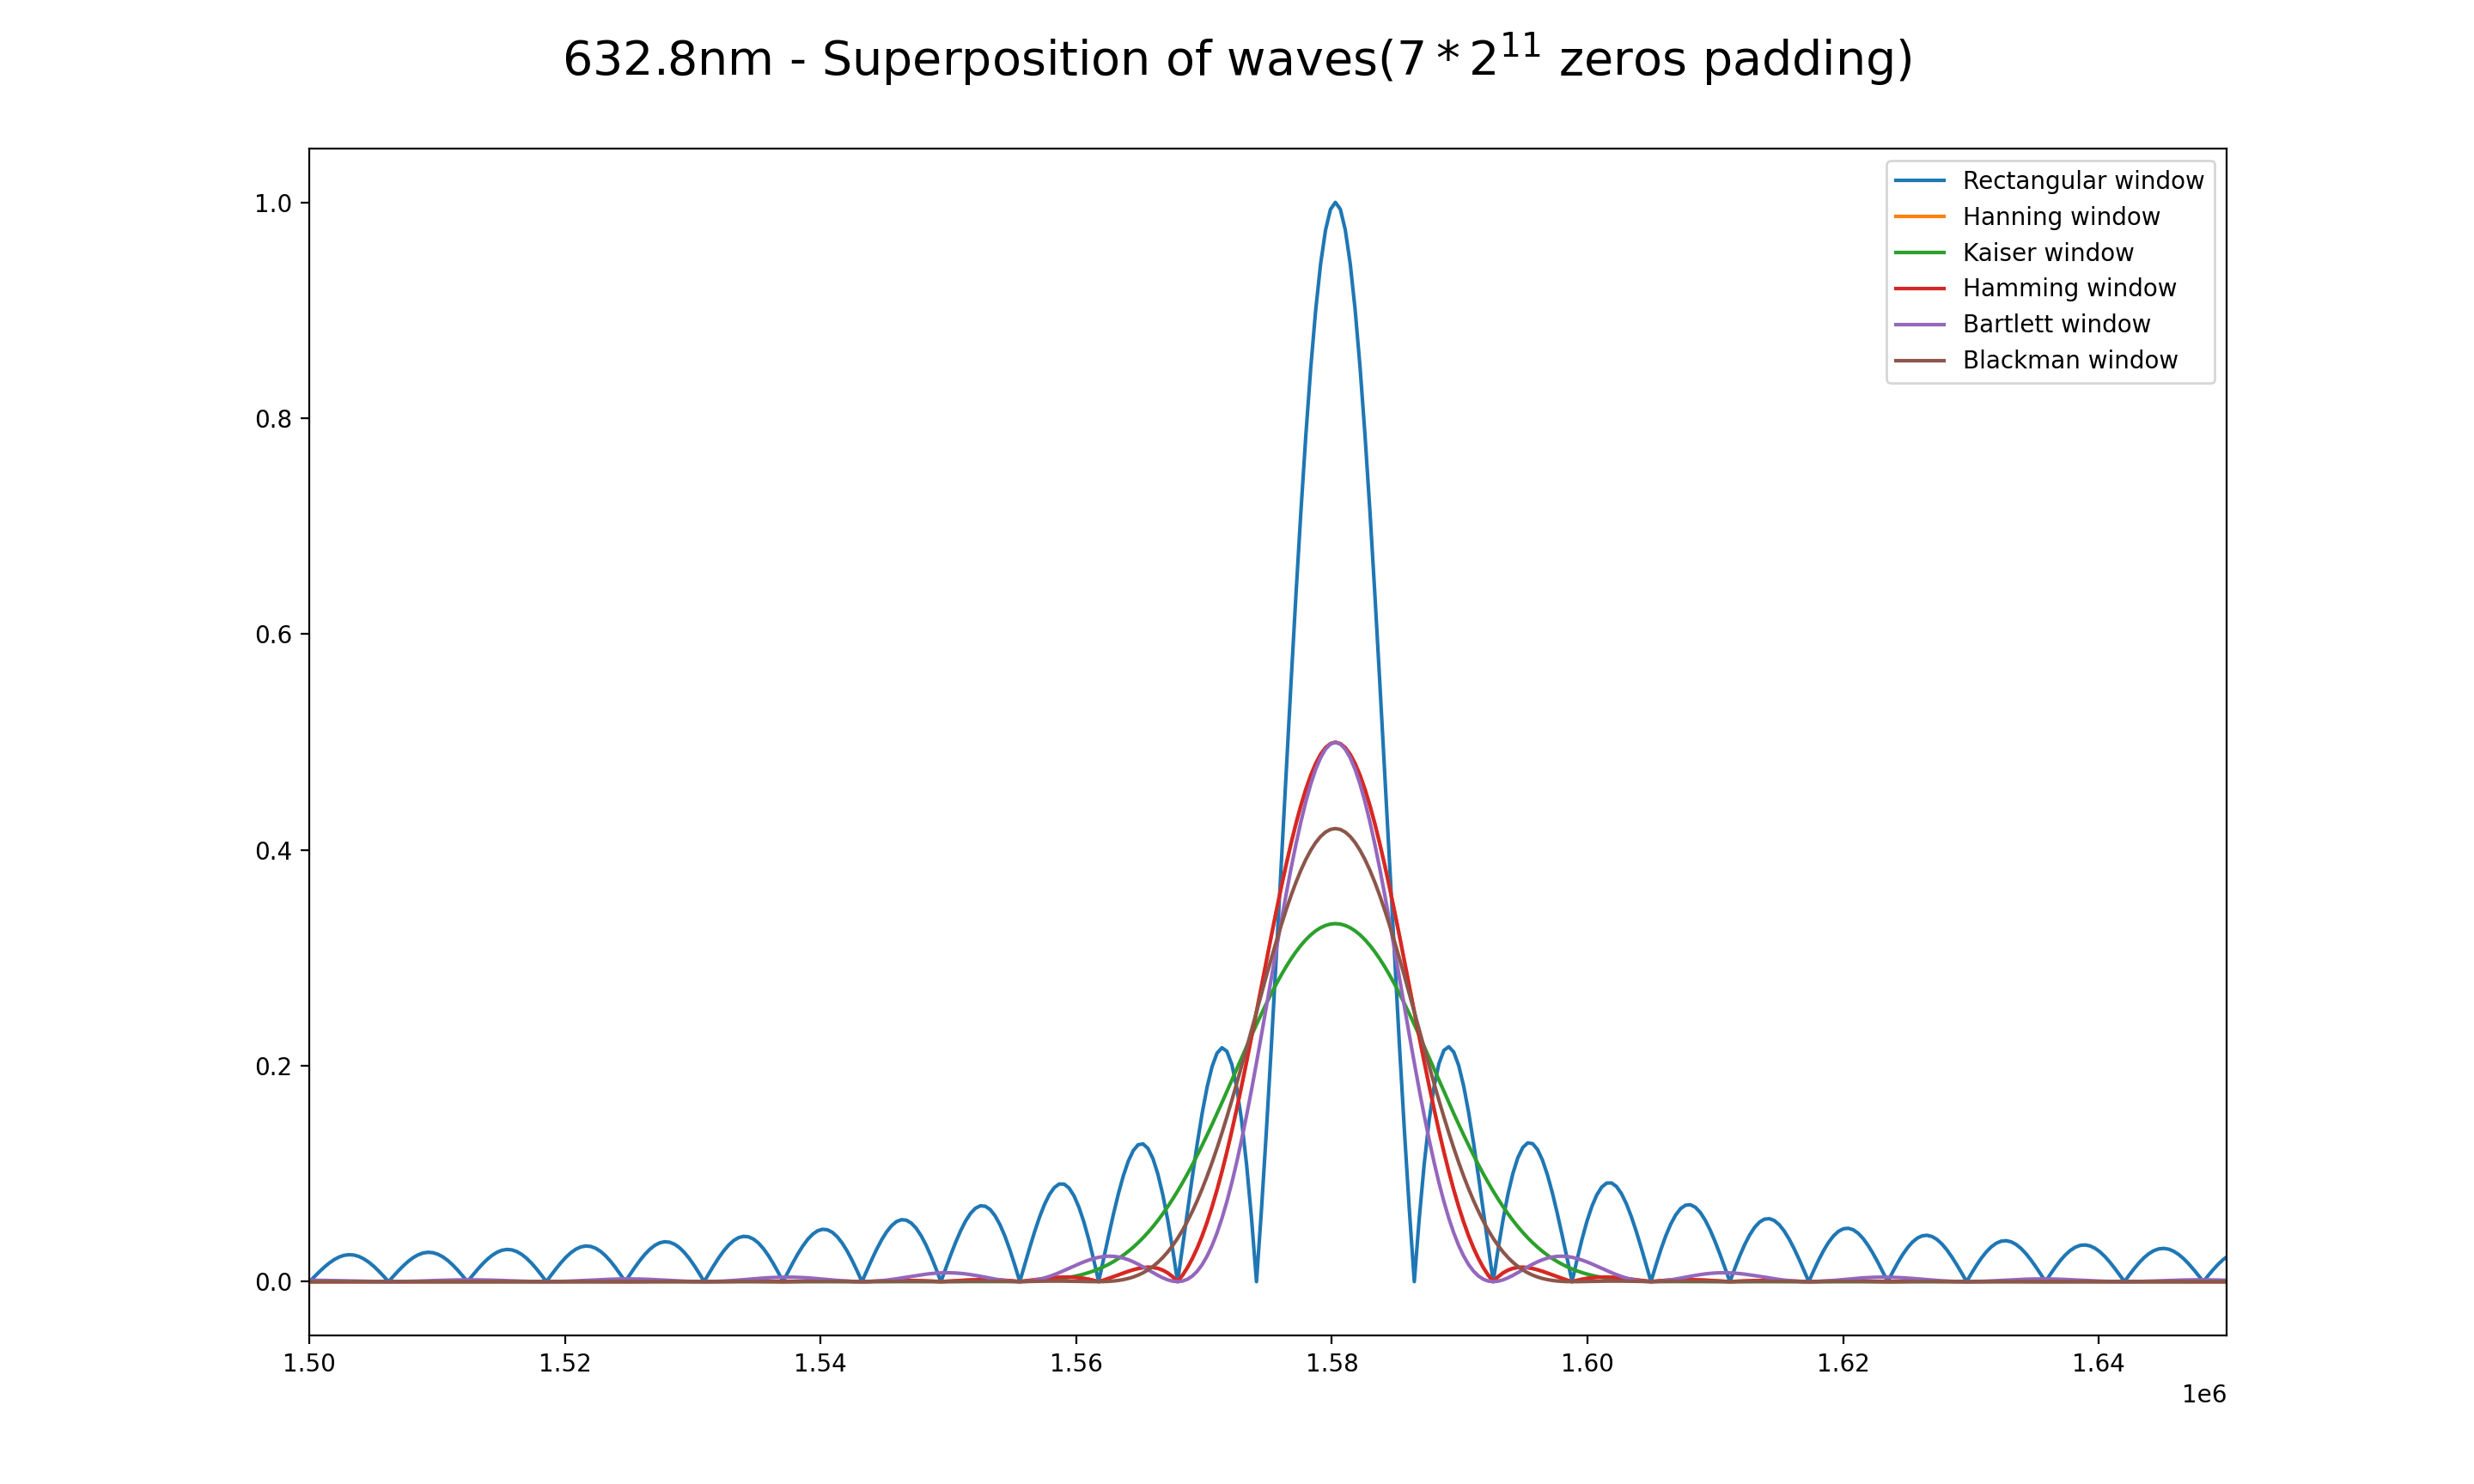
\includegraphics[width=22cm]{pic7.png} 	
	}
	\caption{加窗后与未加窗的FFT曲线的比较}
	\label{pic7}
\end{figure*}

\section{实验结果}

\subsection{加窗实验结果}
图片\ref{pic7}显示了加窗后与未加窗的FFT曲线的比较结果。加窗前与加窗后干涉图补零的个数均为$7\times2^{11}$个。更详细具体的加窗图片如图\ref{pic13}至\ref{pic17}所示,每张图片显示了对干涉图加特殊窗后与对干涉图加矩形窗(未加窗)的比较结果。图片左侧显示了干涉图加窗的波形,右侧图片为FFT曲线的波形,右侧黄色部分的线表示FFT曲线的半波全宽。
\begin{figure}[htbp]
    \centerline{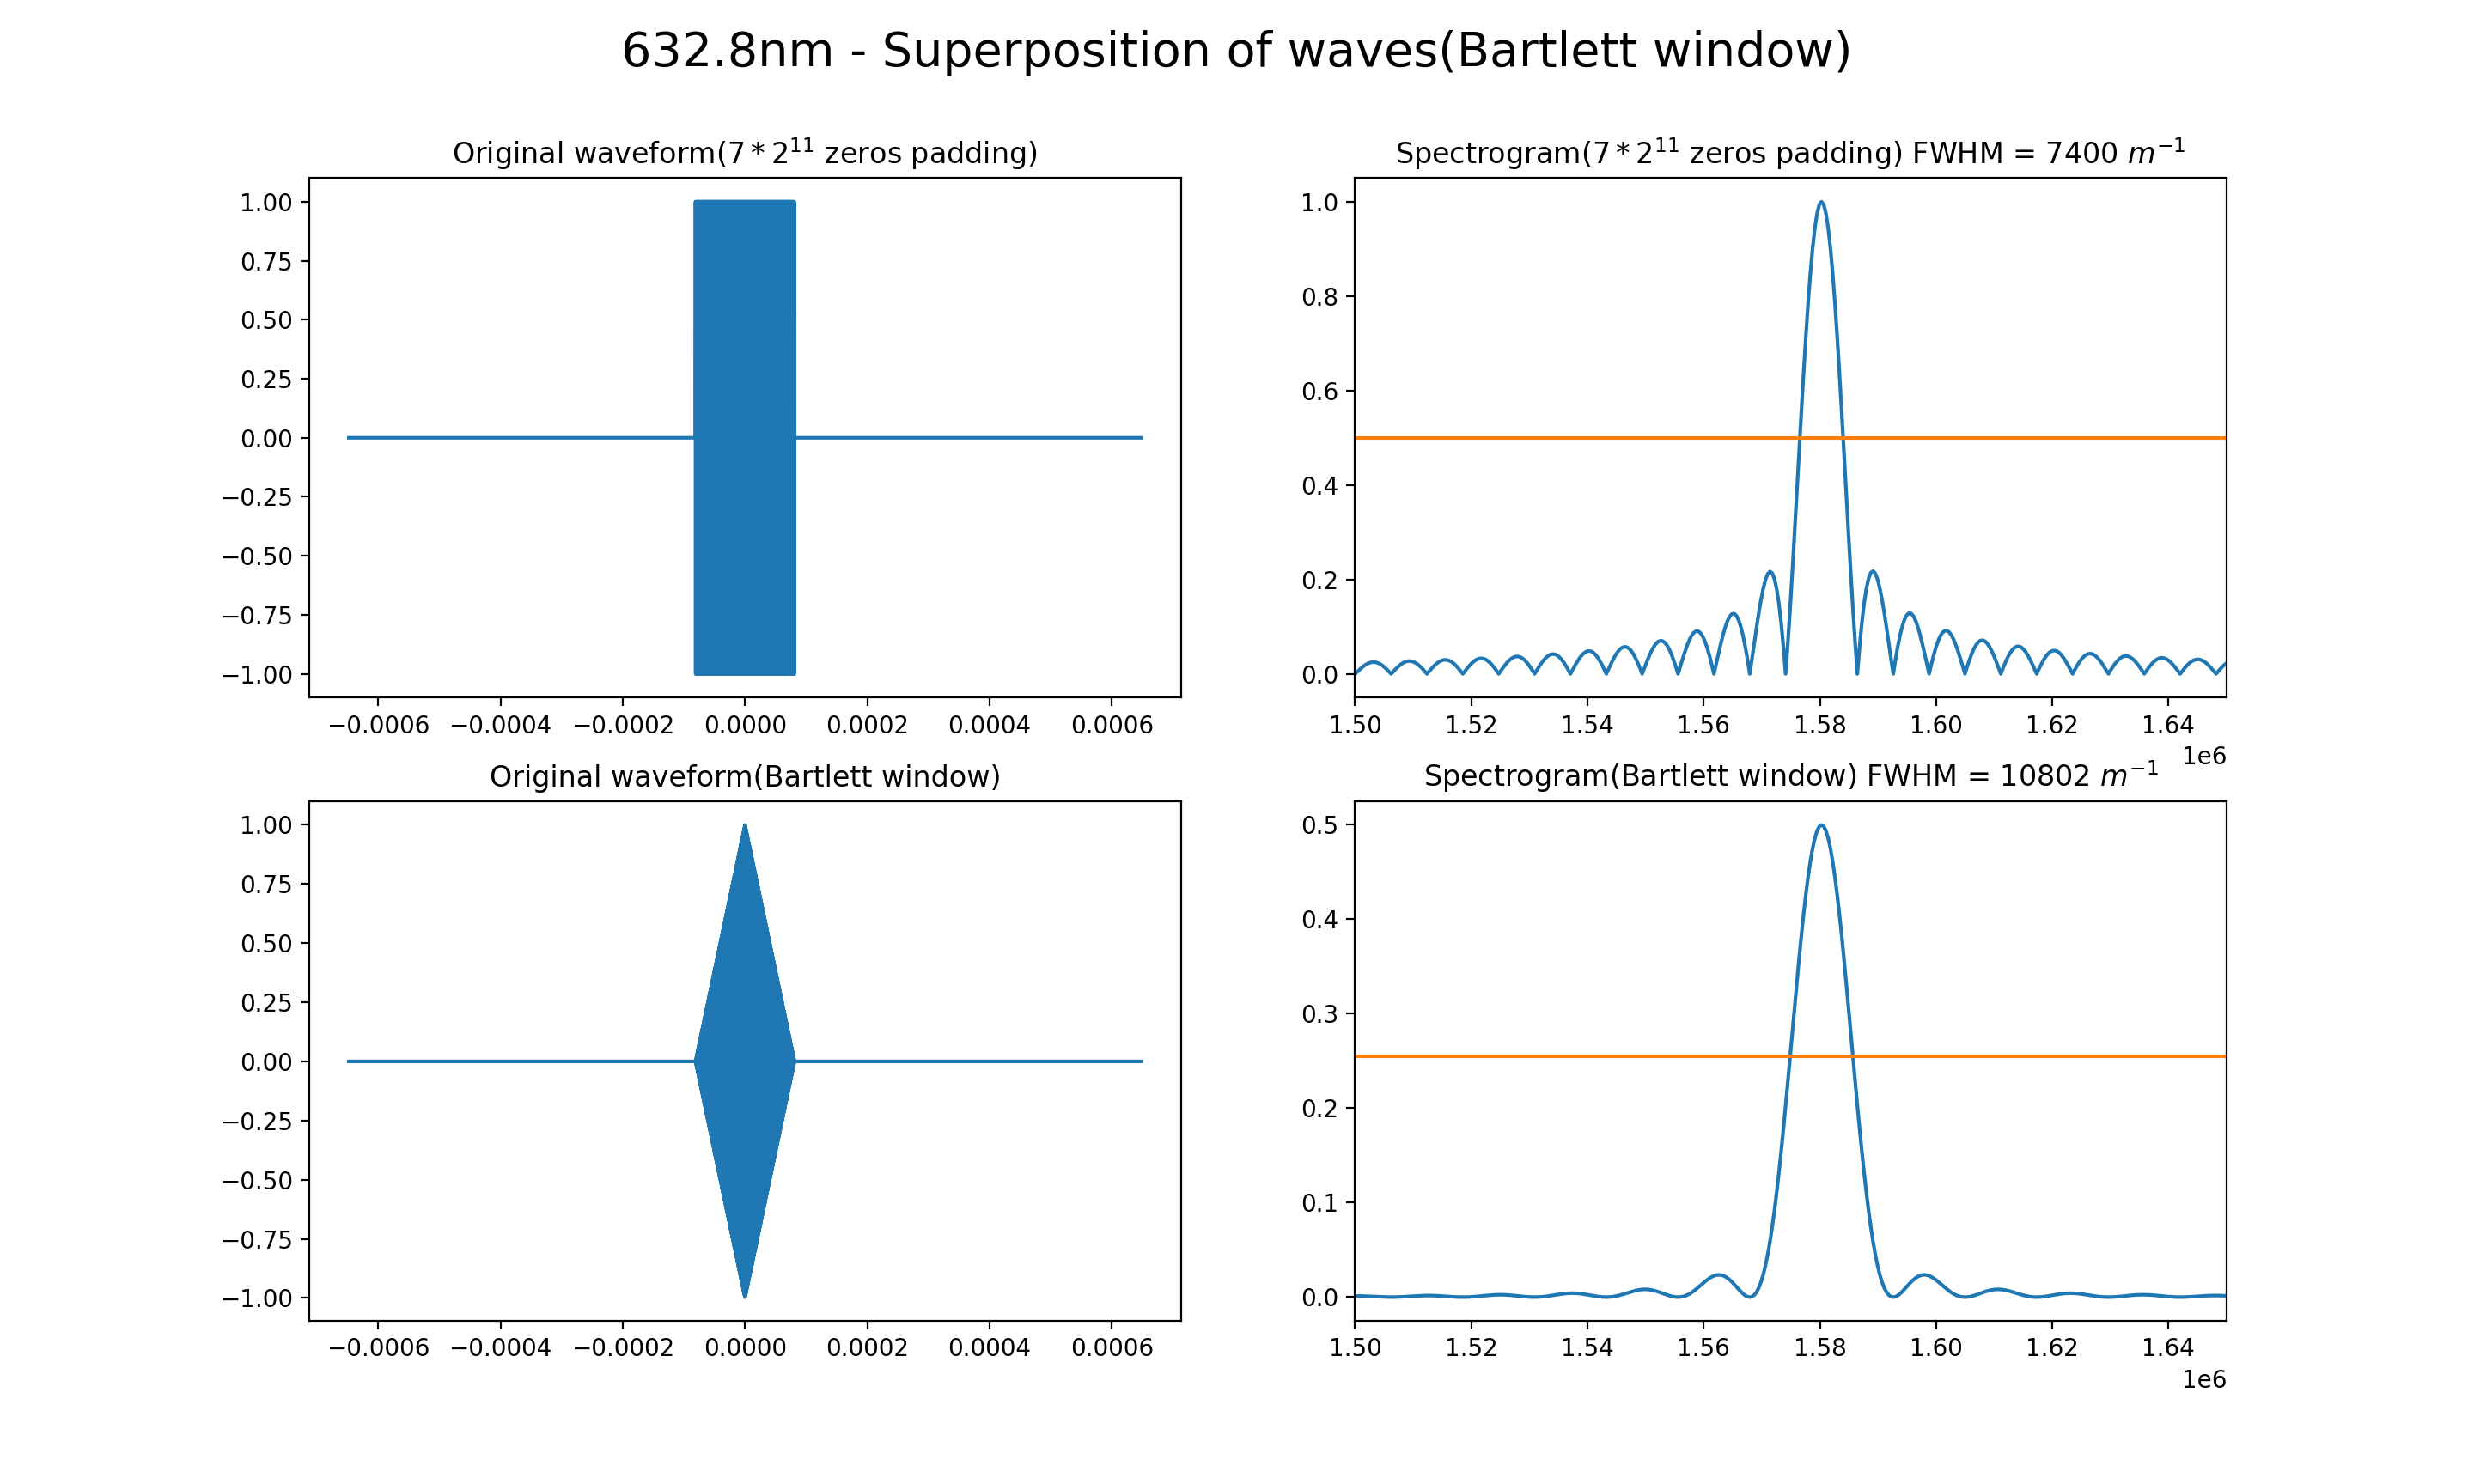
\includegraphics[width=0.5\textwidth]{Bartlett.png}}
    \caption{对干涉图分别加Bartlett窗与矩形窗的比较,图片左侧显示了干涉图加窗的波形,右侧图片为FFT曲线的波形,右侧黄色部分的线表示FFT曲线的半波全宽}
    \label{pic13}
\end{figure}

\begin{figure}[htbp]
    \centerline{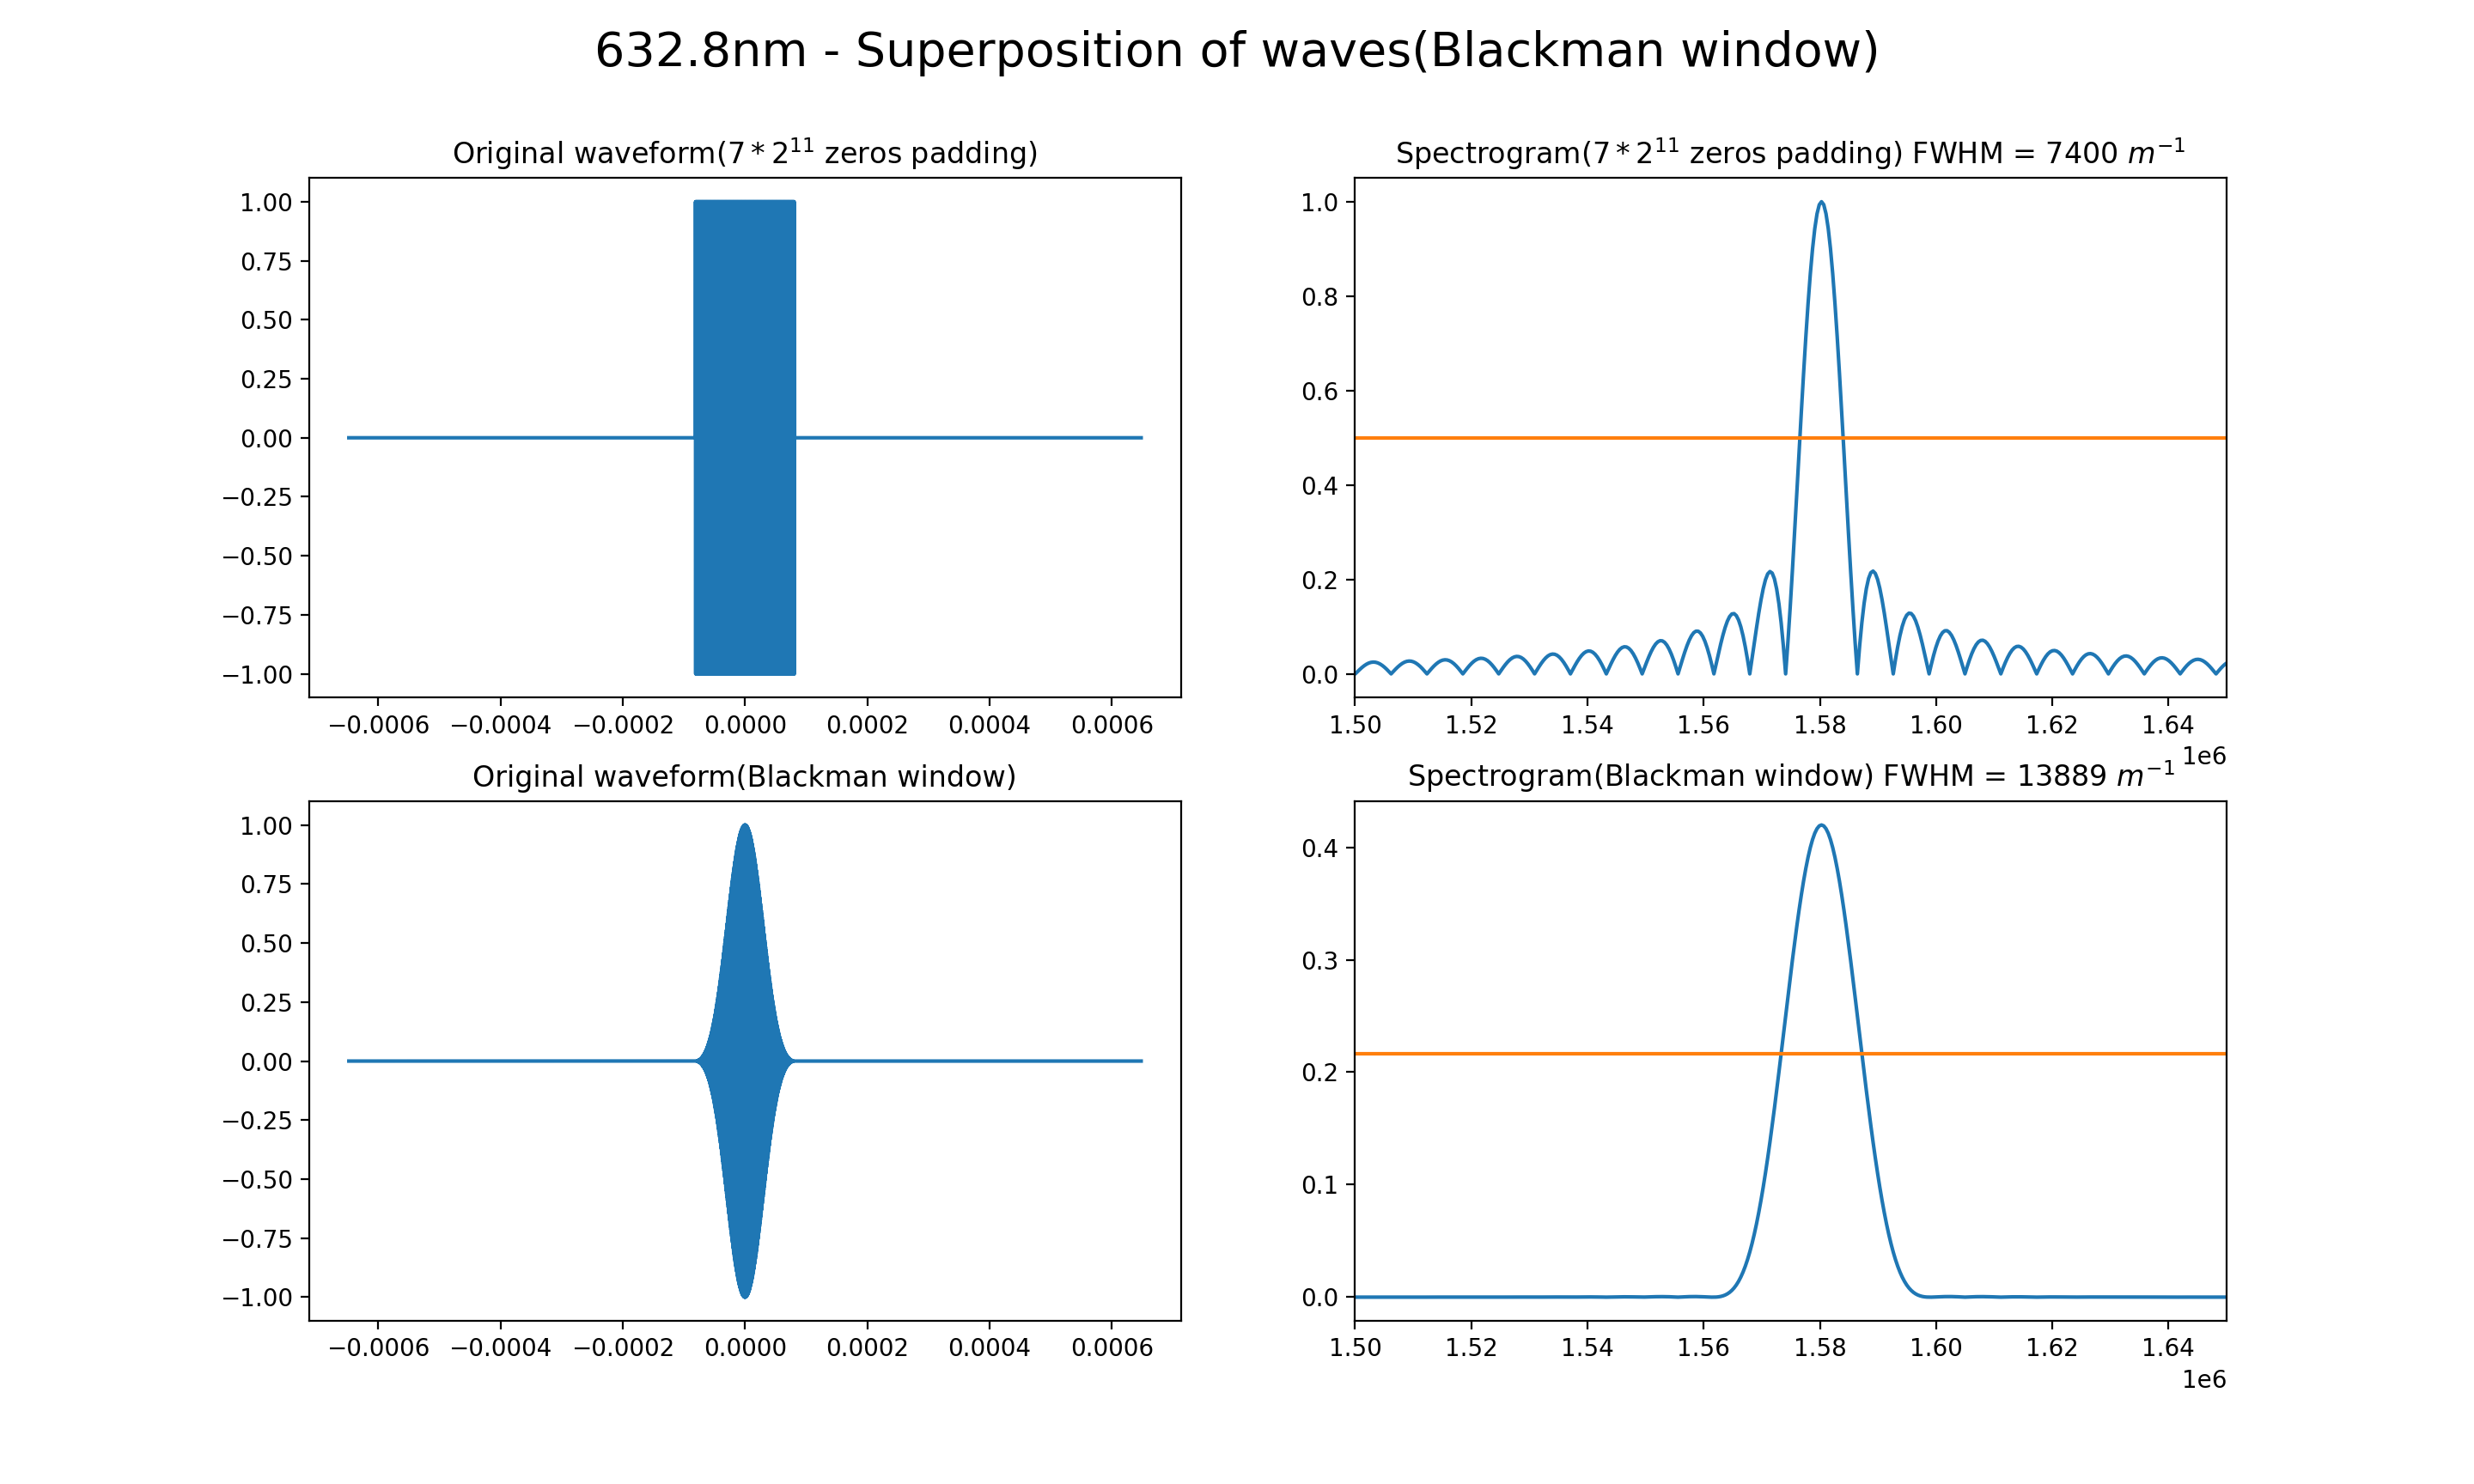
\includegraphics[width=0.5\textwidth]{Blackman.png}}
    \caption{对干涉图分别加Blackman窗与矩形窗的比较,图片左侧显示了干涉图加窗的波形,右侧图片为FFT曲线的波形,右侧黄色部分的线表示FFT曲线的半波全宽}
    \label{pic14}
\end{figure}

\begin{figure}[htbp]
    \centerline{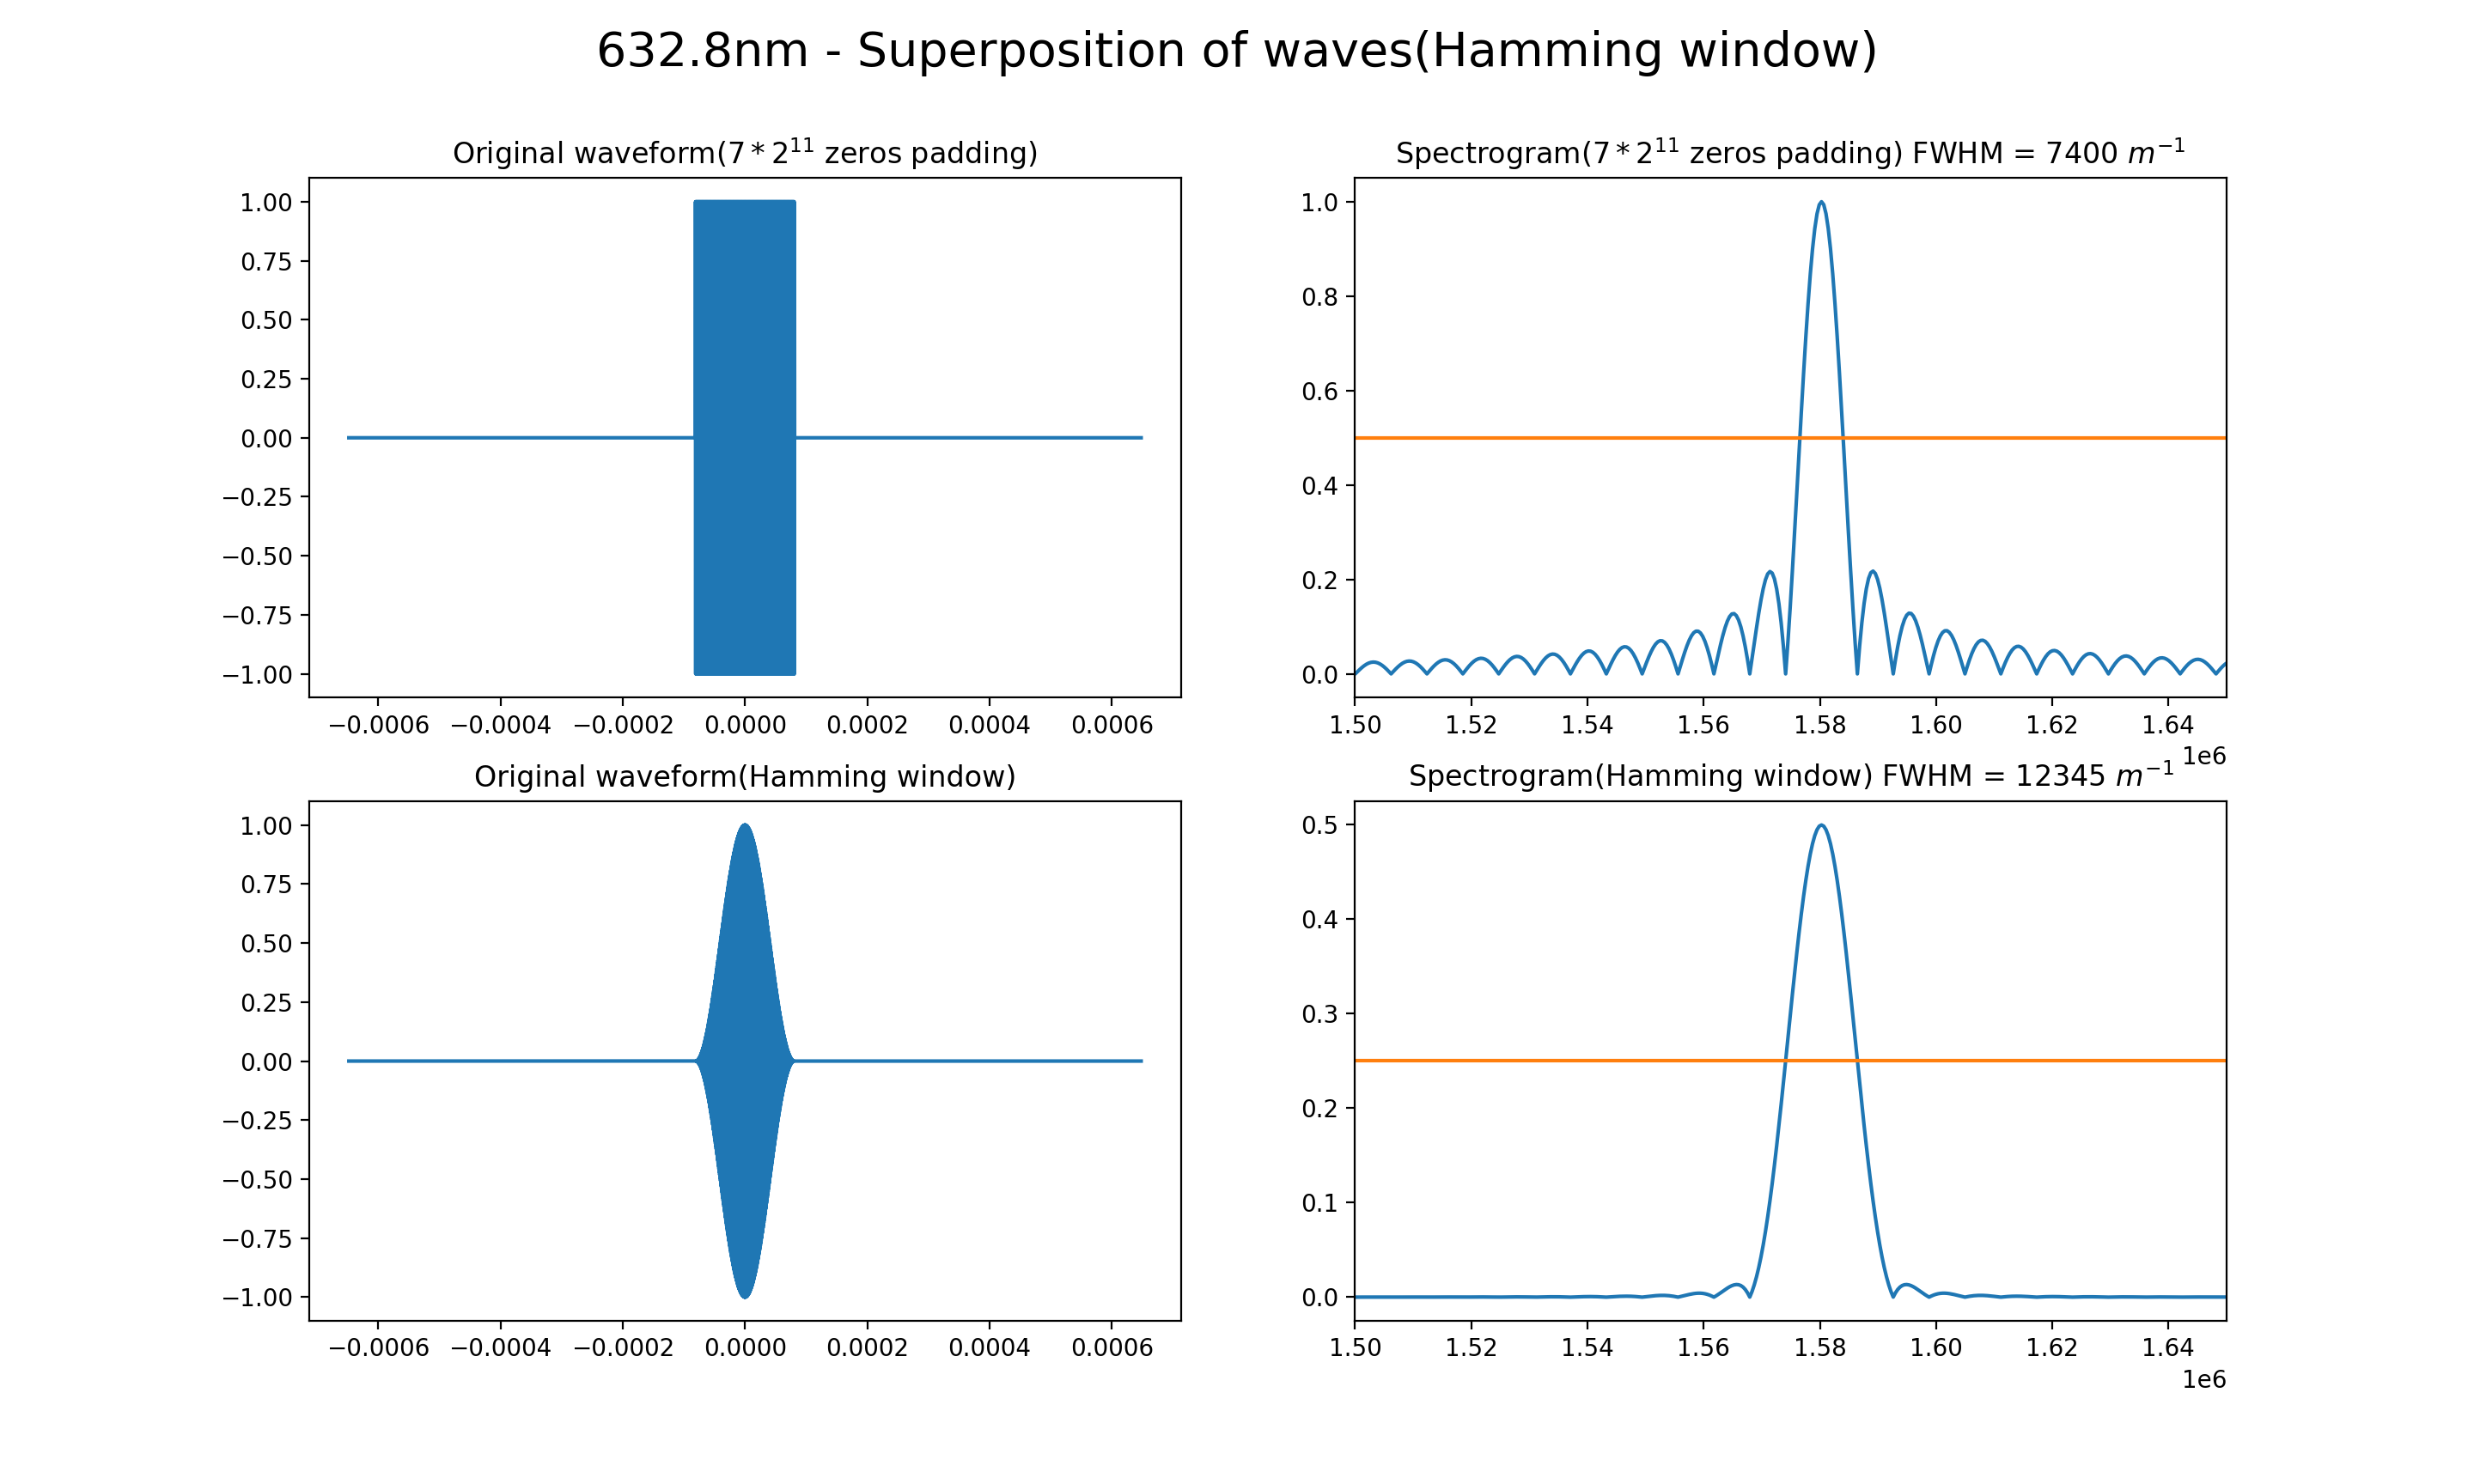
\includegraphics[width=0.5\textwidth]{hamming.png}}
    \caption{对干涉图分别加Hamming窗与矩形窗的比较,图片左侧显示了干涉图加窗的波形,右侧图片为FFT曲线的波形,右侧黄色部分的线表示FFT曲线的半波全宽}
    \label{pic15}
\end{figure}

\begin{figure}[htbp]
    \centerline{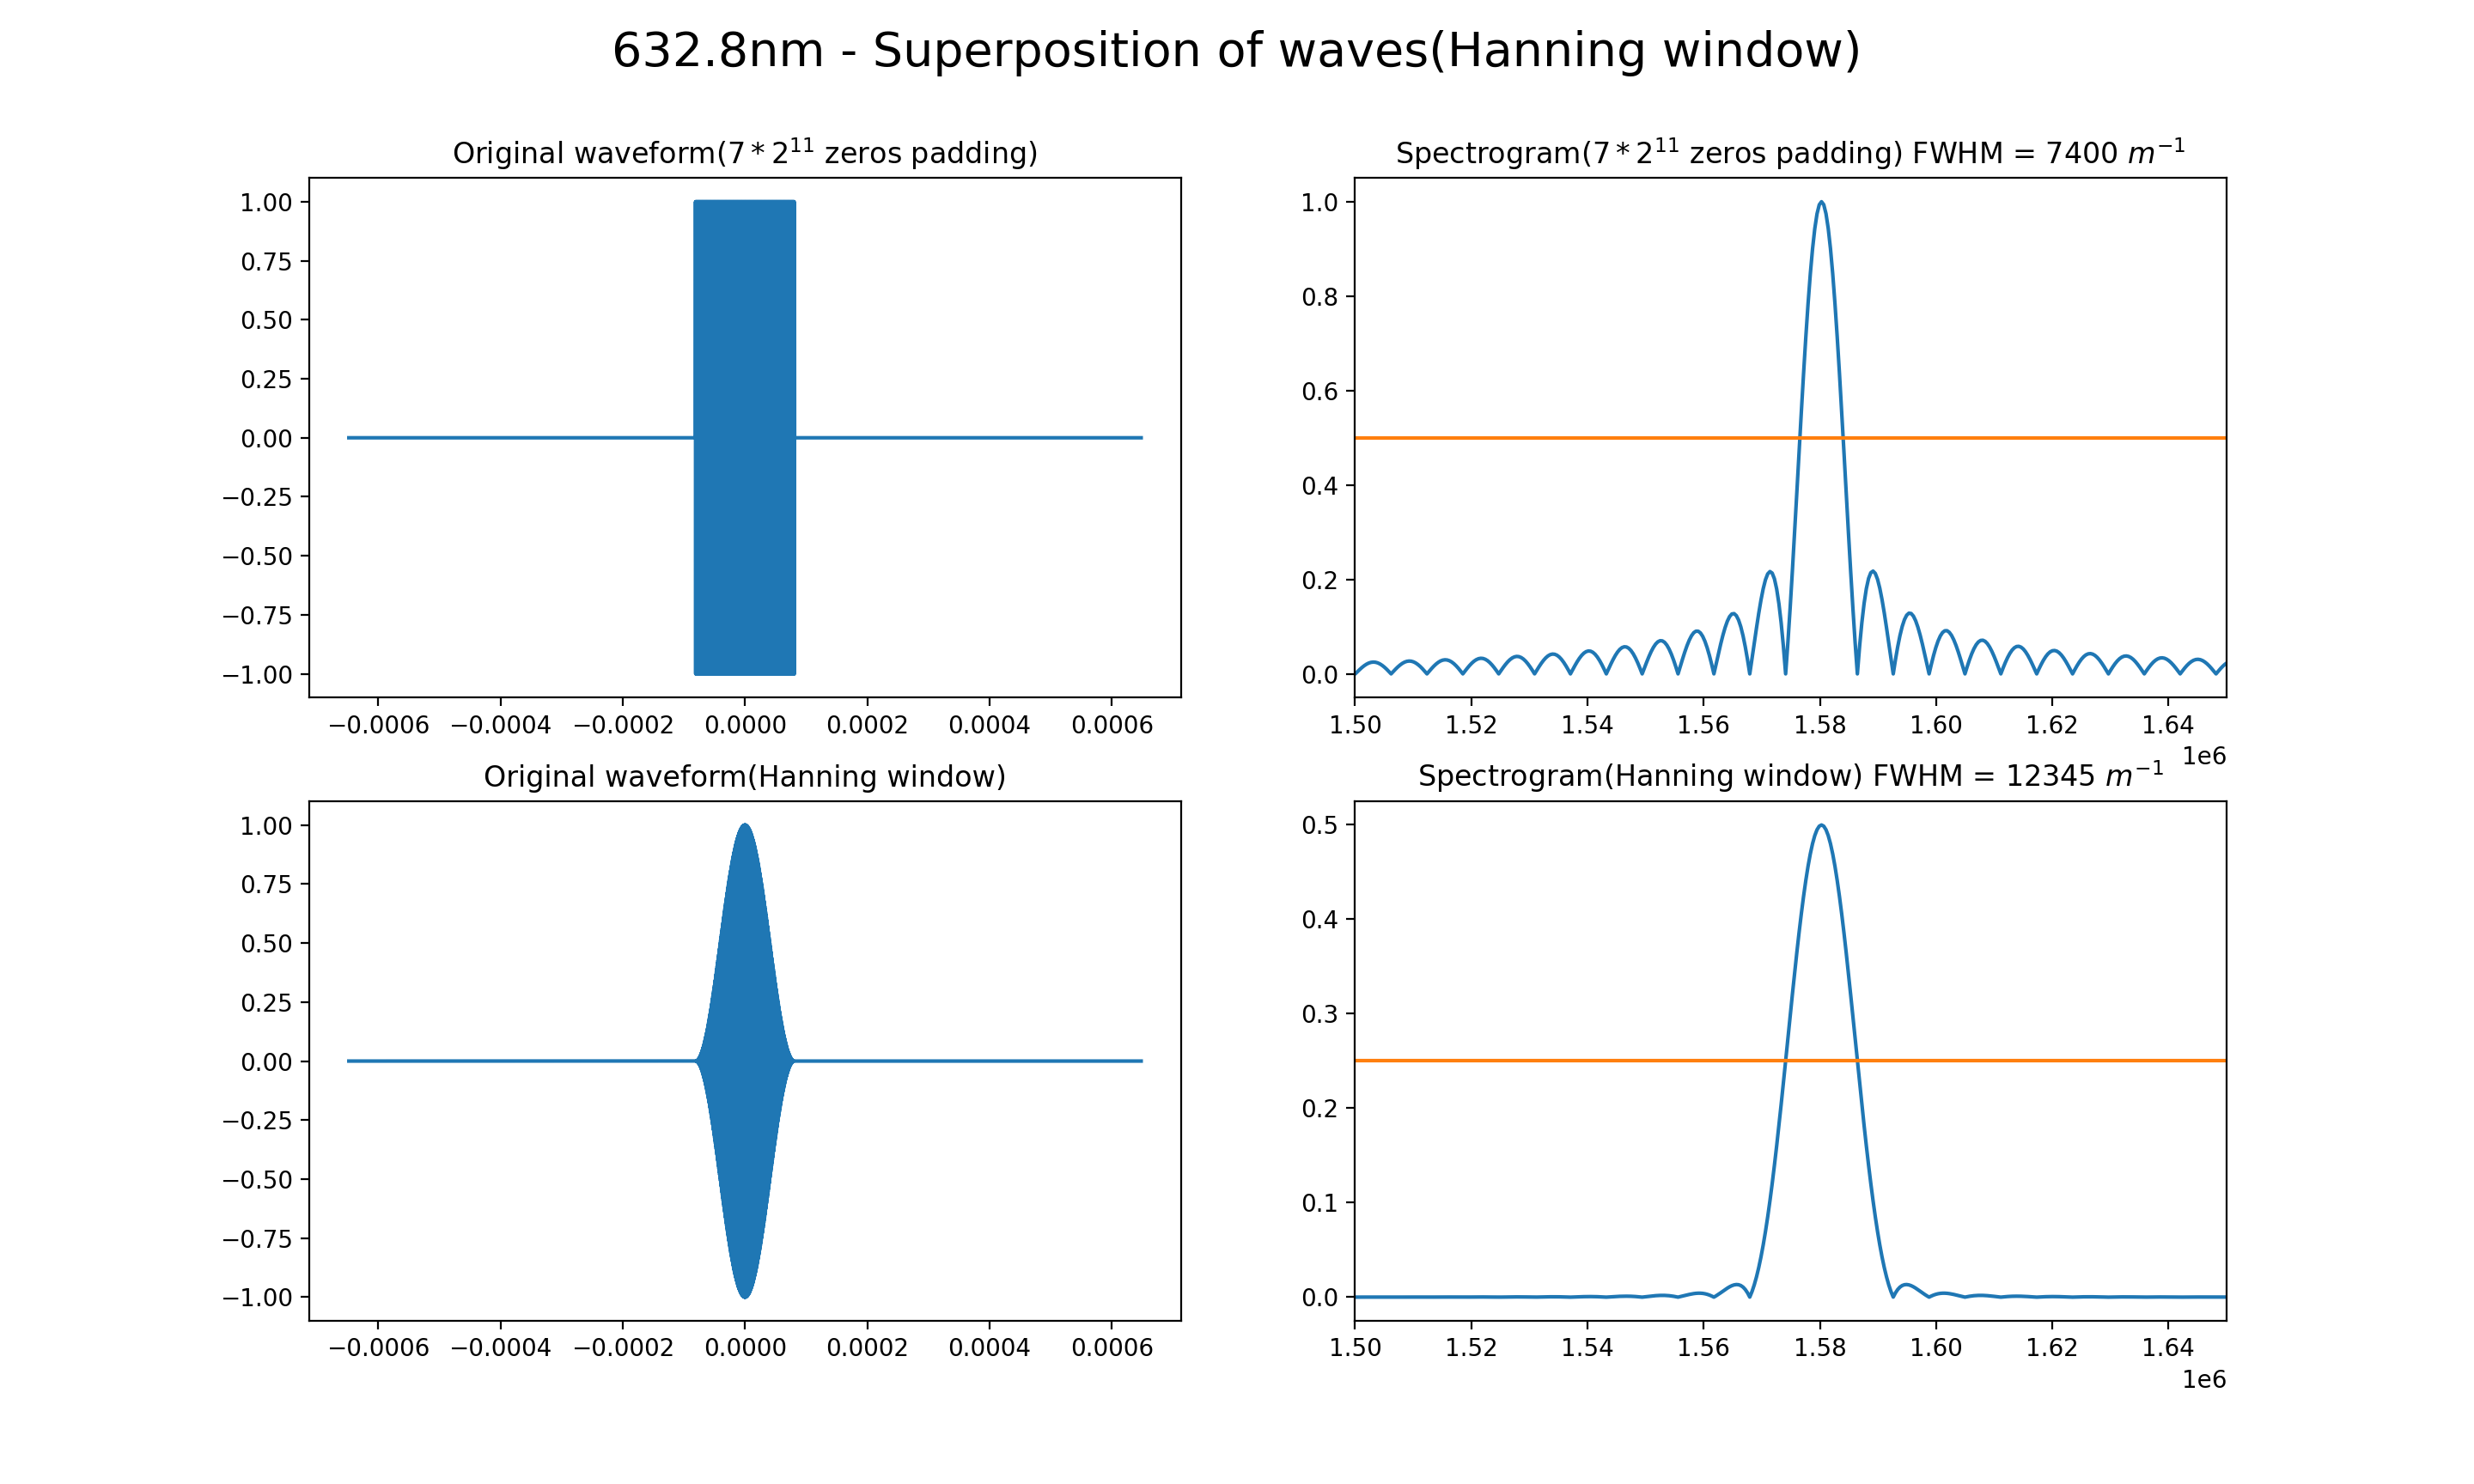
\includegraphics[width=0.5\textwidth]{Hanning.png}}
    \caption{对干涉图分别加Hanning窗与矩形窗的比较,图片左侧显示了干涉图加窗的波形,右侧图片为FFT曲线的波形,右侧黄色部分的线表示FFT曲线的半波全宽}
    \label{pic16}
\end{figure}

\begin{figure}[htbp]
    \centerline{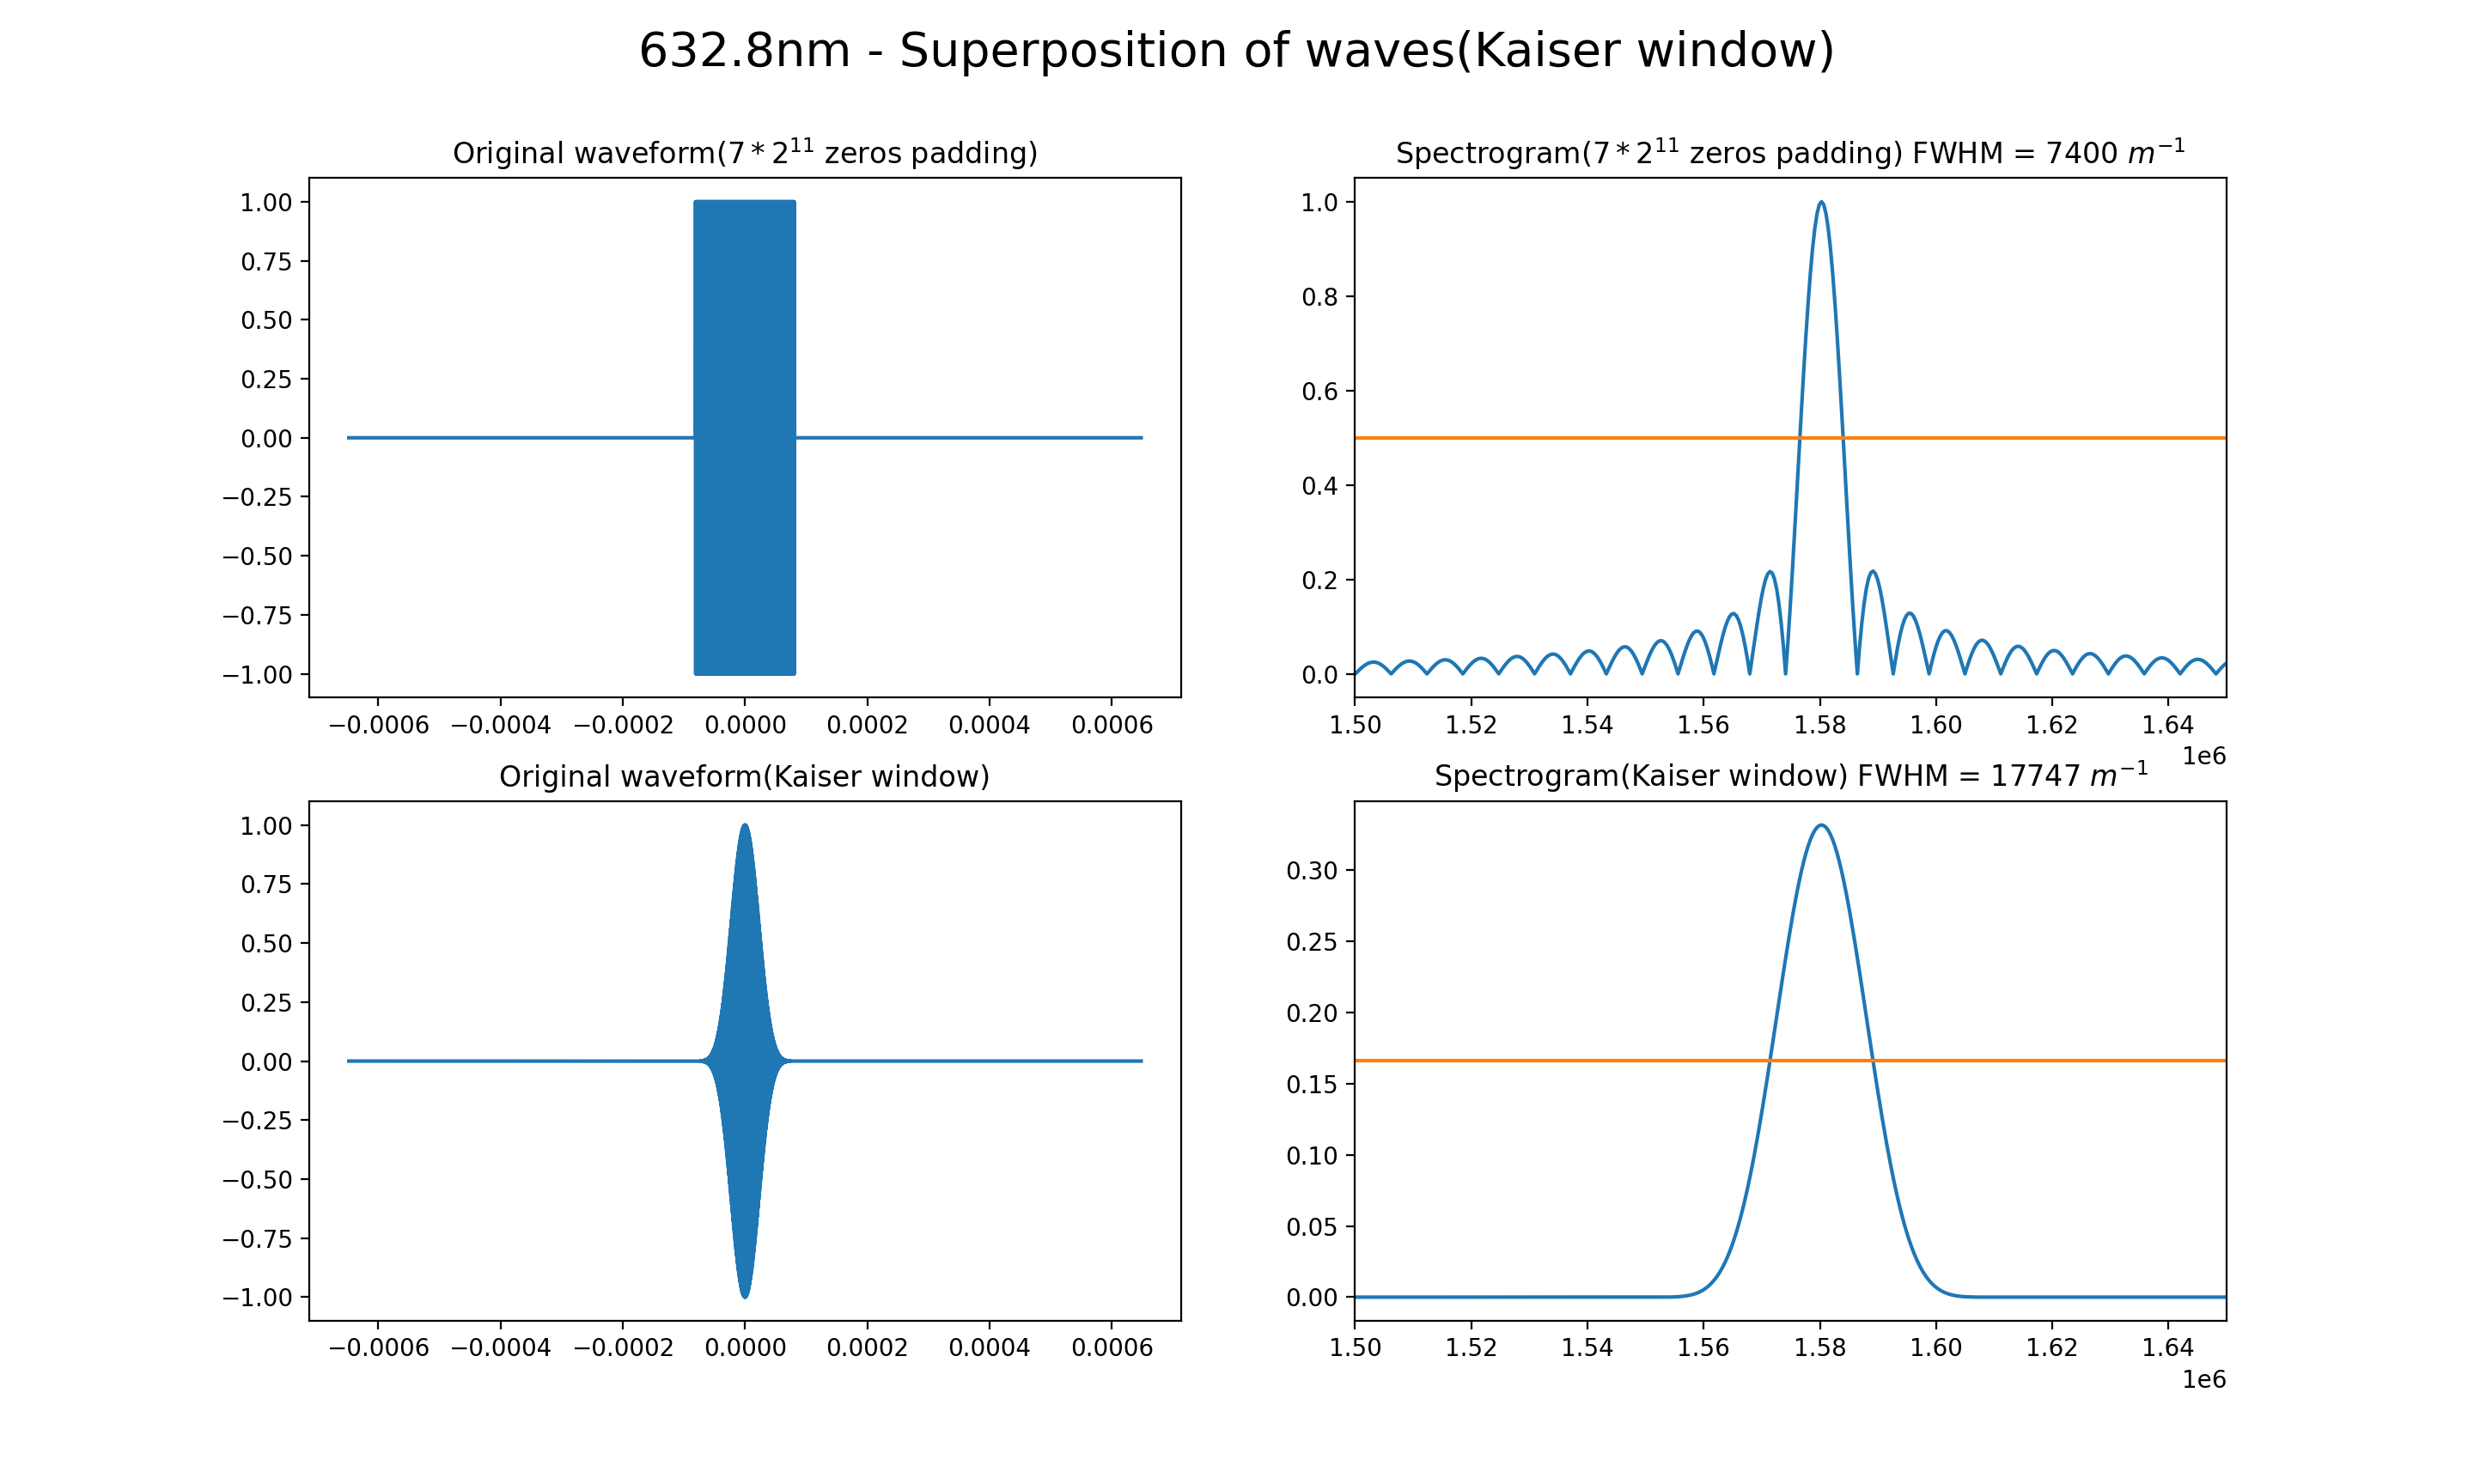
\includegraphics[width=0.5\textwidth]{Kaiser.png}}
    \caption{对干涉图分别加Kaiser窗与矩形窗的比较,图片左侧显示了干涉图加窗的波形,右侧图片为FFT曲线的波形,右侧黄色部分的线表示FFT曲线的半波全宽}
    \label{pic17}
\end{figure}

图\ref{pic13}至\ref{pic17}表明对干涉图加窗函数后将导致原先FFT曲线的幅值部分下降,其中加Kaiser窗对FFT曲线的幅值影响最大,但Kaiser窗对FFT曲线的边频分量的抑制效果最佳。

对干涉图加窗函数还将导致FFT曲线半波全宽变宽的结果。几乎所有窗函数处理后的干涉图的FFT曲线的半波宽度均大于使用矩形窗函数(未加窗)处理后的干涉图的FFT曲线的半波宽度(图片\ref{pic7}),其中加Kaiser窗对FFT曲线的半波宽度影响最大,Hamming窗与Bartlett窗对FFT曲线的半波宽度影响较小,但Bartlett窗对FFT曲线的边频分量的抑制效果较差。

对干涉图加窗函数的优势在于通过加窗后,干涉图对应的FFT曲线的边频分量可以得到有效的抑制。用Kaiser窗处理后的干涉图对应的FFT曲线的边频分量的抑制效果最为明显,Balckman窗处理后的效果次之。

\subsection{补零实验结果}
图片\ref{pic1}显示了补$2^{11}$个零与未补零的FFT曲线的比较结果。图片\ref{pic2}显示了补$3\times2^{11}$个零与未补零的FFT曲线的比较结果。图片\ref{pic3}显示了补$7\times2^{11}$个零与未补零的FFT曲线的比较结果。三个图中,黄色的线代表FFT曲线的半波全宽。

图\ref{pic1},图\ref{pic2}与图\ref{pic3}显示了对干涉图补零不会影响FFT曲线的半波全宽,从频域角度分析,对干涉图补零不会影响频谱的分辨率,补零操作增大了系统的采样点个数,这种操作对FFT分辨率有较好的提升,同时带来了频域波形更加光滑的结果。
\begin{figure}[htbp]
    \centerline{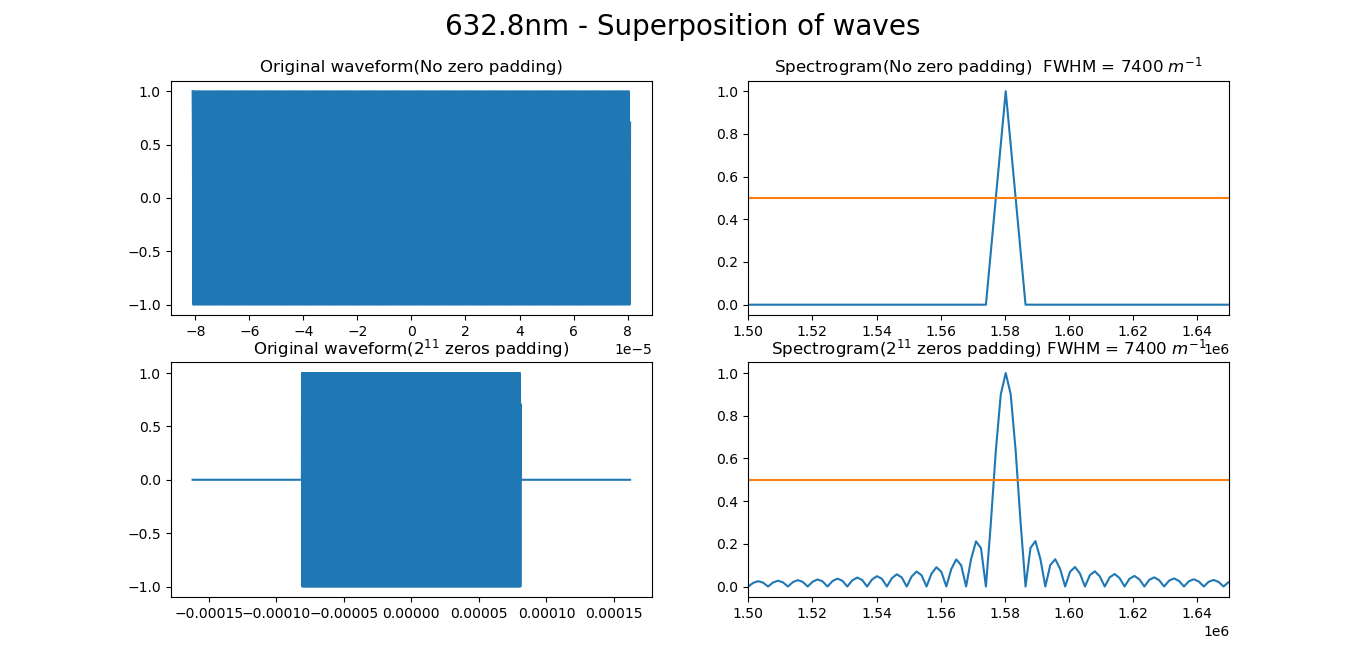
\includegraphics[width=0.5\textwidth]{pic1.png}}
    \caption{补$2^{11}$个零与未补零FFT曲线的比较}
    \label{pic1}
\end{figure}

\begin{figure}[htbp]
    \centerline{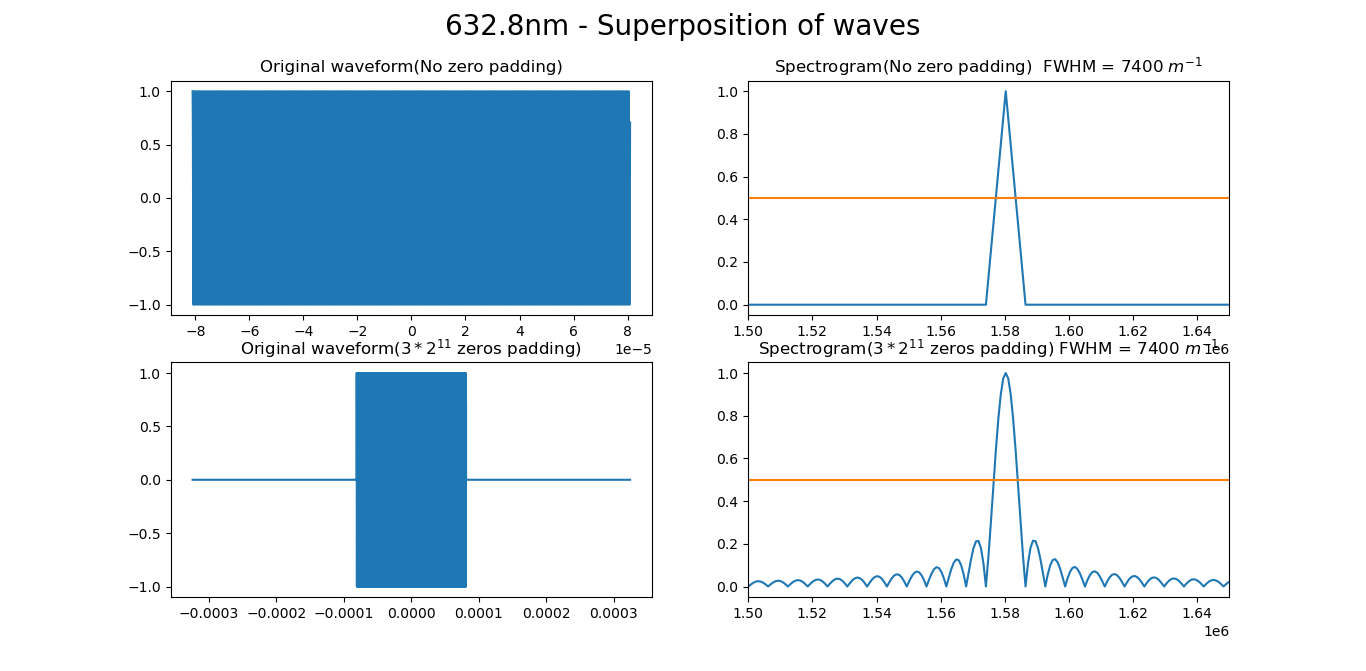
\includegraphics[width=0.5\textwidth]{pic2.png}}
    \caption{补$3\times2^{11}$个零与未补零FFT曲线的比较}
    \label{pic2}
\end{figure}

\begin{figure}[htbp]
    \centerline{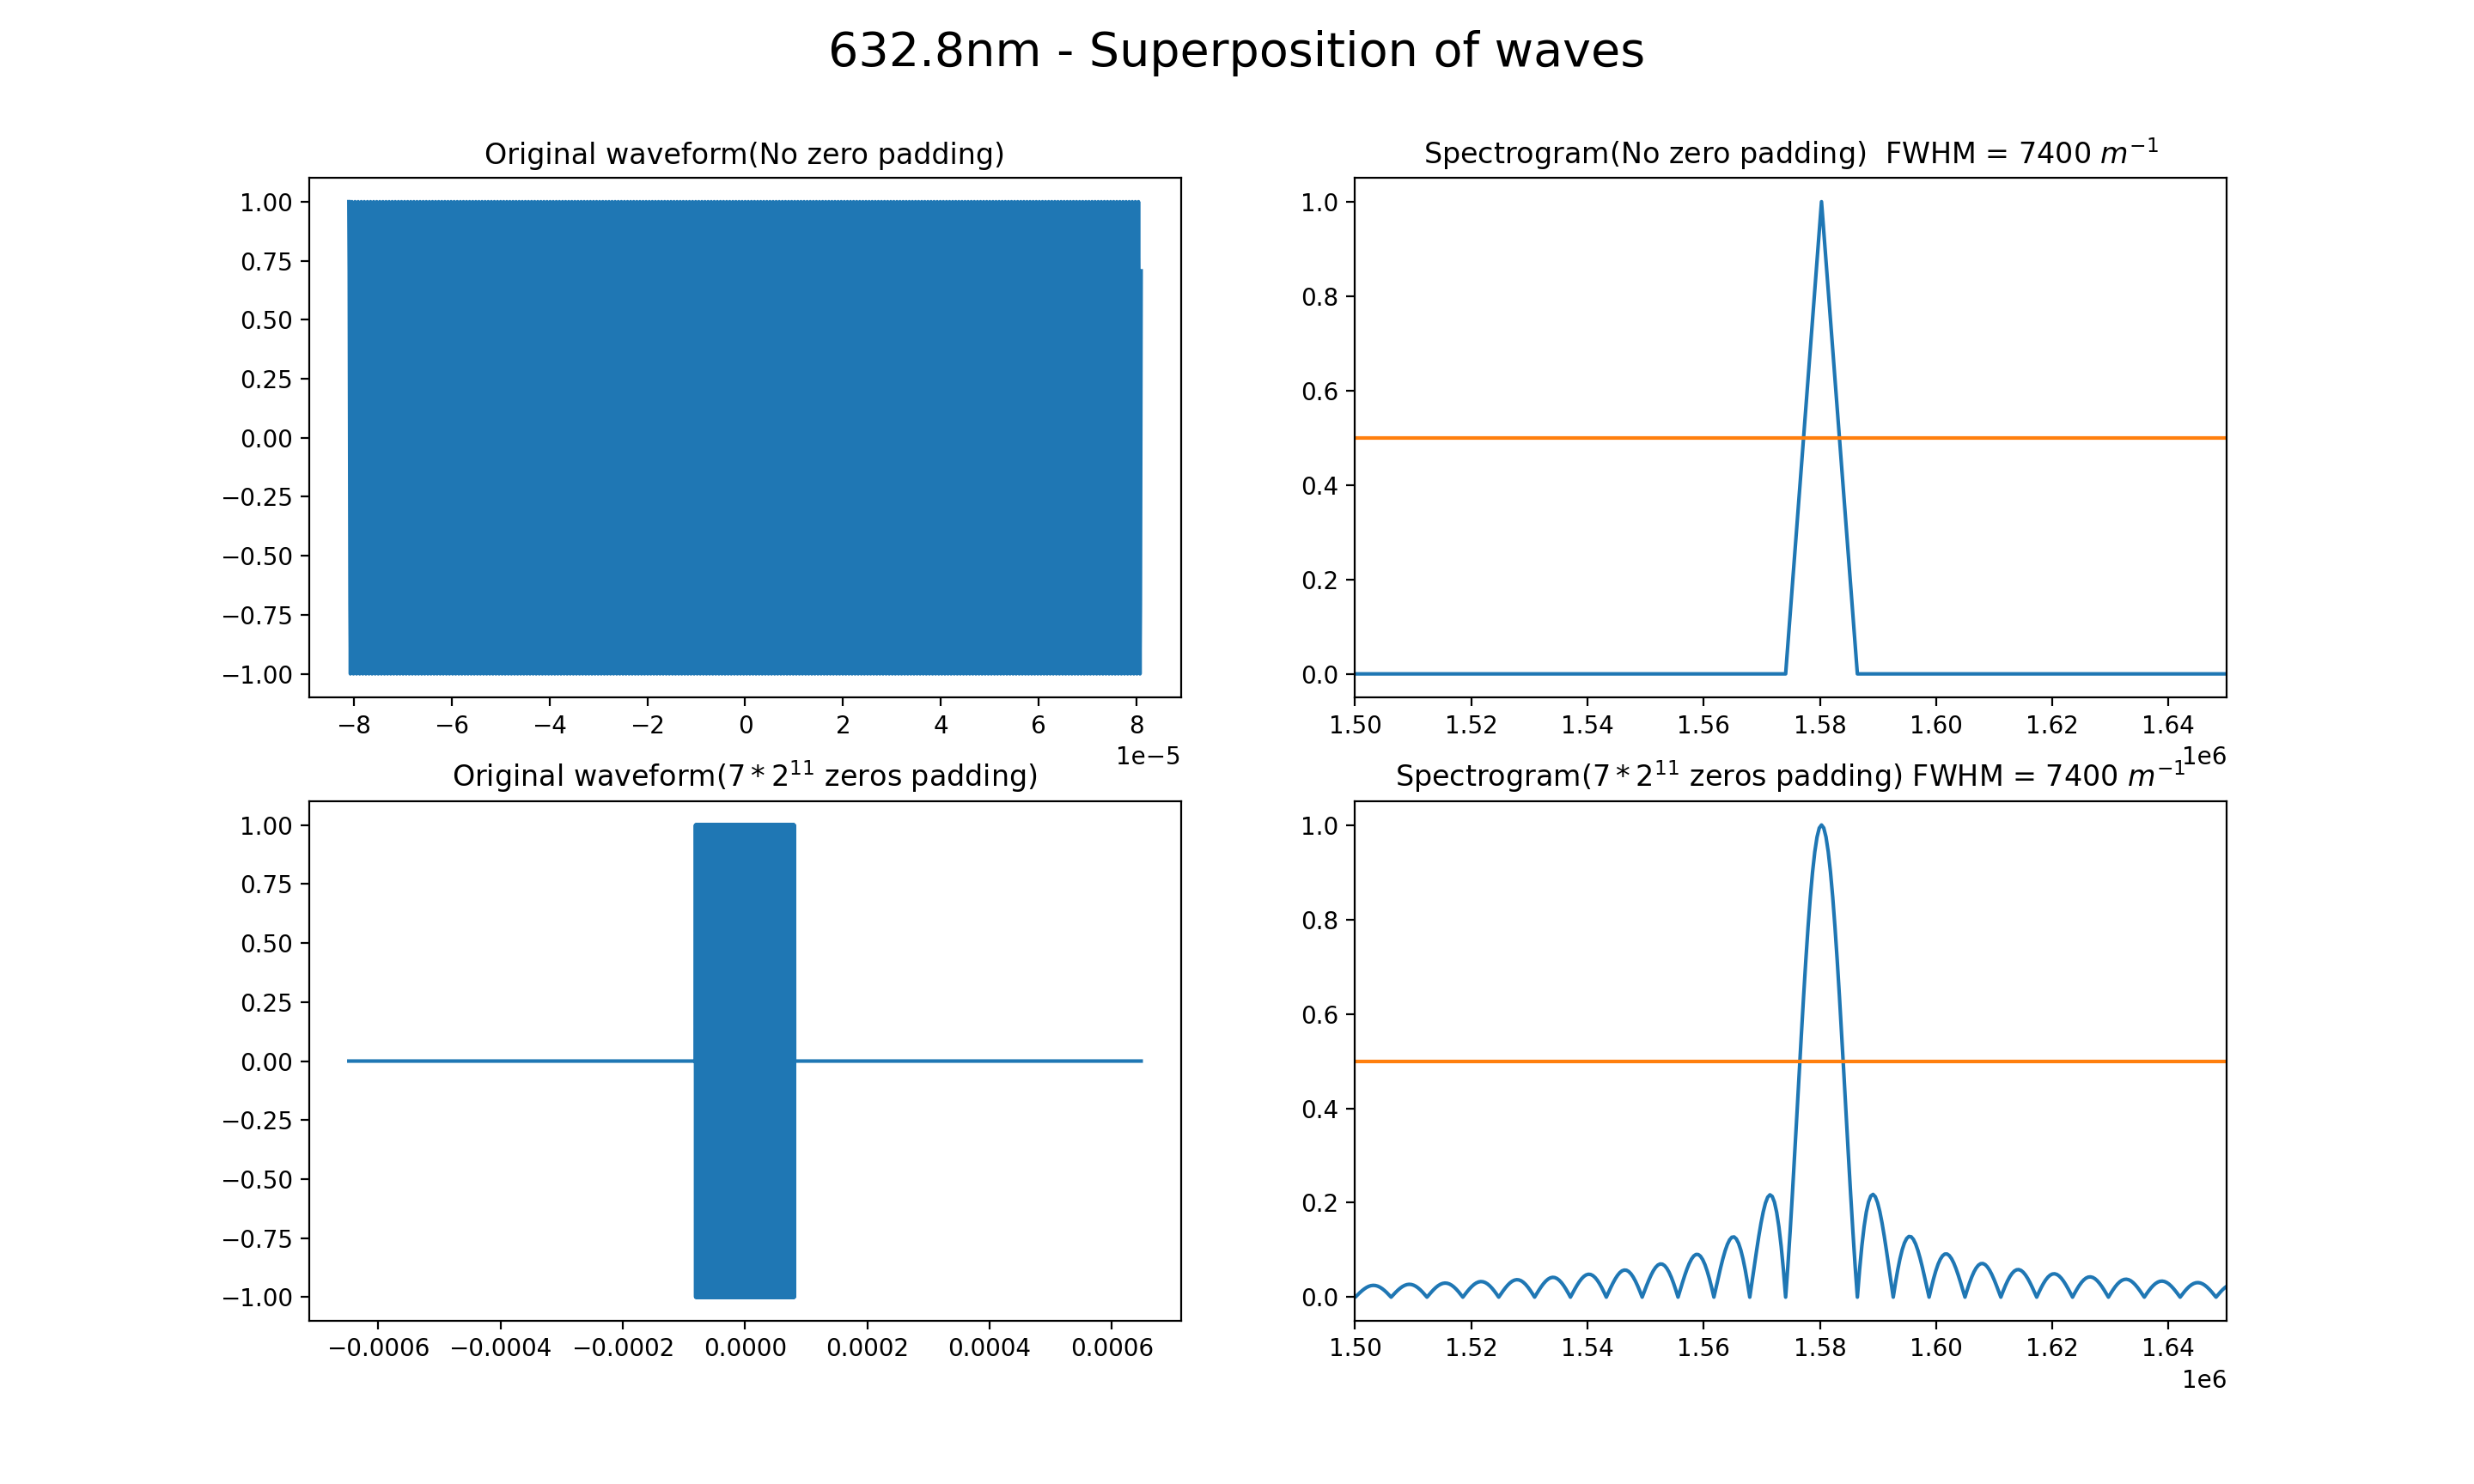
\includegraphics[width=0.5\textwidth]{pic3.png}}
    \caption{补$7\times2^{11}$个零与未补零FFT曲线的比较}
    \label{pic3}
\end{figure}

\subsection{仿真结论}
通过上述对仿真结果的讨论,可以得到如下结论:
\begin{itemize}
    \item[1)] 补0对波形分辨率的几乎没有影响,同时会使旁瓣增多。
    \item[2)] 补0的数量越多,波形越光滑。
    \item[3)] 加窗可以减少旁瓣,但同时使得旁瓣的能量集中到主峰上,因此主峰的波形分辨率变差。
\end{itemize}



\section{结语}
本实验完成了利用Python分别仿真对干涉图补零与对干涉图加窗两因素影响下的傅里叶变换光谱测量系统的FFT曲线的实验。

\end{document}
